

\section{Introduction}
The aim of this project is to create a model of Pentium IV adder in order to estimate its area, delay and power comsumption. For this purpose, a Matlab script has been implemented to derive and plot results. Simulations for 8, 12, 16, 20, 24, 28 and 32 bit cases are reported in this work.\\
In this project it has been supposed that any elementary logic gate necessary are available as external components. Each logic gate is assumed to be already characterized in terms of area, delay, input capacitances and leakage currents.\\
The approach for the design is structural: each block in the pentium IV is characterized like a black-box with its area, delay and power consumption. In this way the internal structure of any block can be changed without modifying anything else and then the Matlab script can be run with the previous settings. This could be very useful to make future improvements for more complex simulations and structural designs.\\



\section{Library logic gates}
The logic gates used in the Pentium IV adder are NAND2, NOR2, INV, XOR2 and the transmission gate (called for brevity "tgate"). In the table  \ref{library_logic_gates} are listed the gates with their parameters.

\begin{table}[H]
\begin{center}
\begin{tabular}{|c|c|c|c|c|}
\hline
GATE & AREA & INPUT & DELAY & AVERAGE LEAKAGE \\
TYPE &      & CAPACINTANCES &  & CURRENT \\ \hline
NAND2 & $A_{nand2}$ & $C_{in_{nand2}}$ & $\tau_{int_{nand2}}+\alpha_{nand2}\cdot C_L$ & $I_{leak_{nand2}}$ \\ \hline
NOR2 & $A_{nor2}$ & $C_{in_{nor2}}$ & $\tau_{int_{nor2}}+\alpha_{nor2}\cdot C_L$ & $I_{leak_{nor2}}$ \\ \hline
INV & $A_{inv}$ & $C_{in_{inv}}$ & $\tau_{int_{inv}}+\alpha_{inv}\cdot C_L$ & $I_{leak_{inv}}$ \\ \hline
XOR2 & $A_{xor2}$ & $C_{in_{xor2}}$ & $\tau_{int_{xor2}}+\alpha_{xor2}\cdot C_L$ & $I_{leak_{xor2}}$ \\ \hline
TGATE & $A_{tgate}$ & $C_{in1_{tgate}}, C_{in2_{tgate}}, C_{in3_{tgate}}$ & $\tau_{int_{tgate}}+\alpha_{tgate}\cdot C_L$ & $I_{leak_{tgate}}$ \\ \hline
\end{tabular}
\end{center}
\caption{library logic gates}
\label{library_logic_gates}
\end{table}

A brief explanation of the parameters is given before the adder analysis. For instance, the NAND2 gate can be considered. \\
$A_{nand2}$ is the area of the NAND2.\\
$I_{leak_{nand2}}$ is the average leakage current of the NAND2. The leakage current of a logic gate depends on the values of its inputs, therefore the average leakage current is a function of the input probabilities. For sake of semplicity, the average leakage current is computed by considering the probabilities of the inputs equal.\\
For the input capacitances and the delay of the NAND2 figure \ref{NAND2_gate} can be considered.

\begin{figure}[H]
\centering
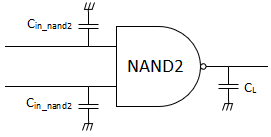
\includegraphics[width = 8cm]{pentium/nand2.png}
\caption{NAND2 gate}
\label{NAND2_gate}
\end{figure}

$C_{in_{nand2}}$ is the input capacitance in each input of the NAND2 gate.\\
The total delay of the NAND2 is 
$\tau_{int_{nand2}}+\alpha_{nand2}\cdot C_L$ where $\tau_{int_{nand2}}$ is the intrinsic delay of the NAND2 (the delay without load) while $\alpha_{nand2}\cdot C_L$ is the contribution that depends on the load $C_L$. The coefficient $\alpha_{nand2}$ depends on the sizes of the transistors inside the gate. The larger the transistors are, the smaller the delay is ($\alpha_{nand2}$ is smaller).\\
In the table, TGATE is the transmission gate. We will use the TGATE to make multiplexers. The TGATE is the only one in the table that has input capacitances depending on which input is considered (differently respect to a normal CMOS gate).\\
It is assumed that all the parameters in table  \ref{library_logic_gates} are given externally. In other words, the design is a function of the parameters reported in the table.\\
Also the supply voltage will be a input parameter because it depends on the technology adopted.\\





\section{Important assumptions in the design}\label{ciao}
To evaluate the dynamic power in the design the switching activity $E_{sw}$ for each node of the circuit has been assumed equal to one. This is a very pessimistic case that it will not happen in reality.\\
Evaluate the switching activity in each node is a very complex work. To do it the statistic of the inputs in our pentium IV should be known. Assuming $E_{sw}=1$ the dynamic power is therefore overestimated. For instance, the real value could be also one order of magnitude smaller. This means that the value of the dynamic power can be considered as an upper bound.\\
The working frequency that it has been used for the dynamic power is the inverse of the critical path of the Pentium IV adder (obviously the clock to output delay of a flip-flop, the setup time and the skew should be considered but this is also a simple estimation for power).\\
The leakage current in table \ref{library_logic_gates} is in the case that the input probabilities for each gate are the same as already said. Obviously this is not true in reality, therefore the value obtained for the static power will be not exactly. However the order of magnitude is expected reasonably correct. This simplification is done because it is too complex to obtain the real statistic of the inputs of each gate: several simulations should be performed in order to obtain the switching activity of each node.\\
To compute the delay of a path, all the delays of all gates in that particular path are summed. This means that, in table \ref{library_logic_gates}, the $50\%$ delay for each gate has been considered.





\section{Pentium IV adder design}
The 32-bit Pentium IV adder is constituted by two blocks as reported in figure \ref{pentiumIV}. The carry-merge sparse tree computes the carry bit in position 4, 8, 12, 16, 20, 24, 28 and 32. The carry-select sum generator computes the sum bit.\\
\begin{figure}[H]
\centering
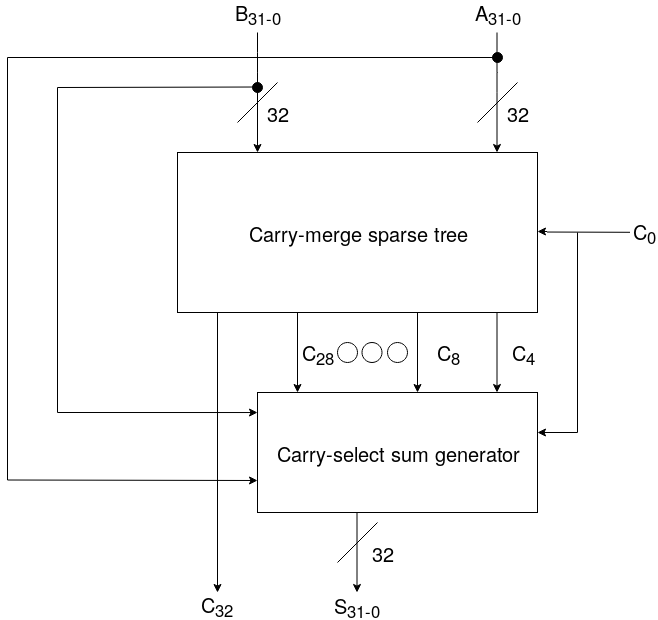
\includegraphics[width = 10 cm]{pentium/pentiumIV.png}
\caption{Pentium IV adder}
\label{pentiumIV}
\end{figure}
In the following sections these two blocks will be detailed. A bottom-up approach has been used to complete this design.





\subsection{Carry-select sum generator design}
In this subsection the carry-select sum generator is designed. 


\subsubsection{Full adder}
In Figure \ref{fa_black_box} it is shown the symbol of the full adder while in Figure \ref{fa_interno} its internal circuit is shown.


\begin{figure}[H]
\centering
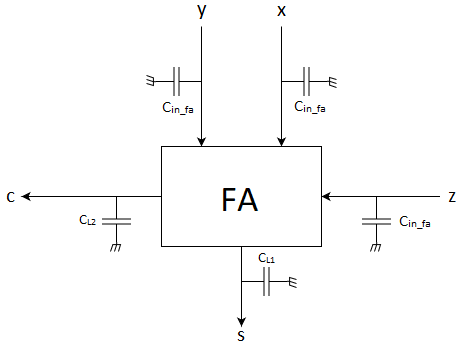
\includegraphics[width = 8cm]{pentium/fa_black_box.png}
\caption{Symbol of full adder}
\label{fa_black_box}
\end{figure}

\begin{figure}[H]
\centering
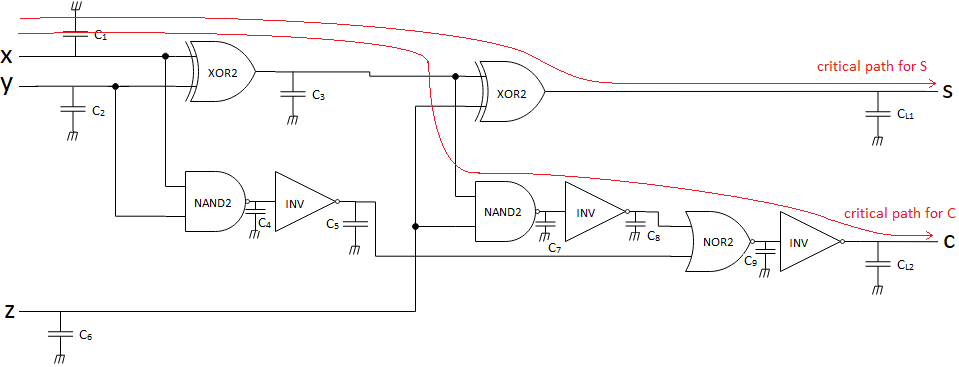
\includegraphics[width = 14cm]{pentium/fa_interno.png}
\caption{Internal full adder circuit}
\label{fa_interno}
\end{figure}

The full adder area is given by:
\begin{equation}
A_{FA}=2A_{xor2}+2A_{nand2}+A_{nor2}+3A_{inv}
\end{equation}
The leakage current is:
\begin{equation}
I_{leak_{FA}}=2I_{leak_{xor2}}+2I_{leak_{nand2}}+I_{leak_{nor2}}+3I_{leak_{inv}}
\end{equation}
The static power is:
\begin{equation}
P_{stat_{FA}}=V_{DD}\cdot I_{leak_{FA}}
\end{equation}
For the dynamic power, as said, it has been assumed that the switching activity $E_{sw}$ of all the nodes in the circuit is equal to one. Therefore it is possible to write:
\begin{equation}
P_{dyn_{FA}}=V_{DD}^2f_{CLK}E_{sw}(C_3+C_4+C_5+C_7+C_8+C_9)
\end{equation}
NOTE: for the dynamic power only the internal nodes are considered, which is that the input and output ones are not taken into account. The contribution of the input and output nodes will be considered when the FA-block will be used to create others blocks.\\
Looking at figure \ref{fa_interno} it is possible to see that:
\begin{equation}
C_1=C_2=C_3=C_6=C_{in_{xor2}}+C_{in_{nand2}}
\end{equation}
\begin{equation}
C_4=C_7=C_9=C_{in_{inv}}
\end{equation}
\begin{equation}
C_5=C_8=C_{in_{nor2}}
\end{equation}

Thus:
\begin{equation}
P_{dyn_{FA}}=V_{DD}^2f_{CLK}E_{sw}(C_{in_{xor2}}+C_{in_{nand2}}+3C_{in_{inv}}+2C_{in_{nor2}})
\end{equation}

The intrinsic delay (the delay without load) of the output $S$ is:
\begin{equation}
\tau_{int_{FA_{S}}} = \tau_{int_{xor2}}+\alpha_{xor2}C_3+\tau_{int_{xor2}} = 2\tau_{int_{xor2}}+\alpha_{xor2}(C_{in_{xor2}}+C_{in_{nand2}})
\end{equation}

The $\alpha$ parameter is:
\begin{equation}
\alpha_{FA_{S}}=\alpha_{xor2}
\end{equation}

Thus the total delay of $S$ (considering the load) is $\tau_{int_{FA_{S}}}+\alpha_{FA_{S}}C_{L1}$.\\\\
Analogously for the output $C$ it is obtained:
\begin{equation}
\tau_{int_{FA_{C}}} = \tau_{int_{xor2}}+\alpha_{xor2}C_3+\tau_{int_{nand2}}+\alpha_{nand2}C_7+\tau_{int_{inv}}+\alpha_{inv}C_8+\tau_{int_{nor2}}+\alpha_{nor2}C_9+\tau_{int_{inv}}
\end{equation}

\begin{equation}
\alpha_{FA_{C}}=\alpha_{inv}
\end{equation}

The delay of $C$ considering the load will be $\tau_{int_{FA_{C}}}+\alpha_{FA_{C}}C_{L2}$.\\\\

The input capacitances of the full adder are:
\begin{equation}
C_{in_{x}}=C_{in_{y}}=C_{in_{z}}=C_{in_{FA}}=C_{in_{xor2}}+C_{in_{nand2}}
\end{equation}





\subsubsection{4-bit ripple carry adder}
In Figure \ref{rca4_black_box} it is shown the symbol of the 4-bit ripple carry adder while in Figure \ref{rca4_interno} its internal circuit is shown.


\begin{figure}[H]
\centering
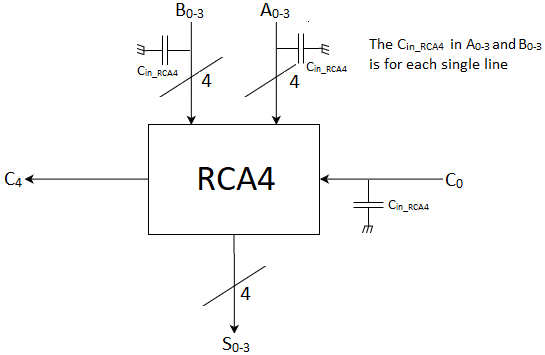
\includegraphics[width = 10cm]{pentium/rca4_black_box.png}
\caption{symbol of 4-bit ripple carry adder}
\label{rca4_black_box}
\end{figure}

\begin{figure}[H]
\centering
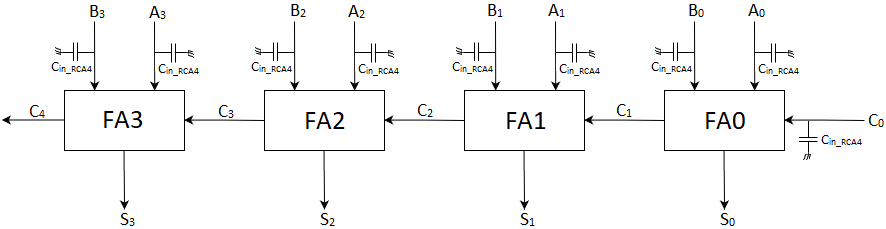
\includegraphics[width = 14cm]{pentium/rca4_interno_copia.png}
\caption{internal circuit of 4-bit ripple carry adder}
\label{rca4_interno}
\end{figure}

The  area of 4-bit ripple carry adder is given by:
\begin{equation}
A_{RCA4}=4A_{FA}
\end{equation}
The leakage current is:
\begin{equation}
I_{leak_{RCA4}}=4I_{leak_{FA}}
\end{equation}
The static power is:
\begin{equation}
P_{stat_{RCA4}}=V_{DD}\cdot I_{leak_{RCA4}}
\end{equation}

Just as in the case of the full adder, in order to compute the dynamic power only the internal nodes have been considered:
\begin{equation}
P_{dyn_{RCA4}}=V_{DD}^2f_{CLK}E_{sw}(3C_{in_{FA}})+4P_{dyn_{FA}}
\end{equation}
NOTE: the term $4P_{dyn_{FA}}$ is for the internal nodes of the FAs.\\\\
To compute the delay, it can be observed that the delay to generate the 4 sum bits ($S_0, S_1, S_2$ and $S_3$) is the main concern. This is why the output carry ($C_4$) will be generated by the tree. Thus the delay of RCA4 to be considered is the delay to generate $S_3$. The intrinsic delay (that without load) can be written as:

\begin{equation}
\tau_{int_{RCA4}} = 3\tau_{int_{FA_{C}}}+\alpha_{FA_{C}}(3C_{in_{FA}})+\tau_{int_{FA_{S}}}
\end{equation}

For the alpha coefficient it is derived that:
\begin{equation}
\alpha_{RCA4}=\alpha_{FA_{S}}
\end{equation}

The input capacitances for the carry input ($C_0$) and for each line of $A_{0-3}$ and $B_{0-3}$ is the same and equal to:
\begin{equation}
C_{in_{RCA4}}=C_{in_{FA}}
\end{equation}





\subsubsection{Transmission gate}
The transmission gate has been used to make multiplexers. Using transmission gates to implement MUXs, instead of normal CMOS gates, is in fact a good solution in terms of area, delay and power consuption.\\
In Figure \ref{tgate_black_box} it is shown the symbol of the transmission gate while in figure \ref{tgate_interno} its internal circuit.

\begin{figure}[H]
\centering
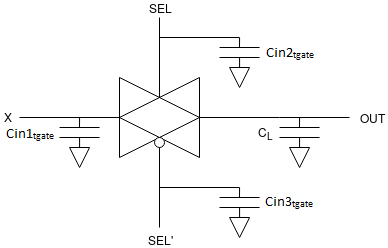
\includegraphics[width = 8 cm, height = 5 cm]{pentium/transmission_gate_black_box.png}
\caption{Symbol of the transmission gate}
\label{tgate_black_box}
\end{figure}

\begin{figure}[H]
\centering
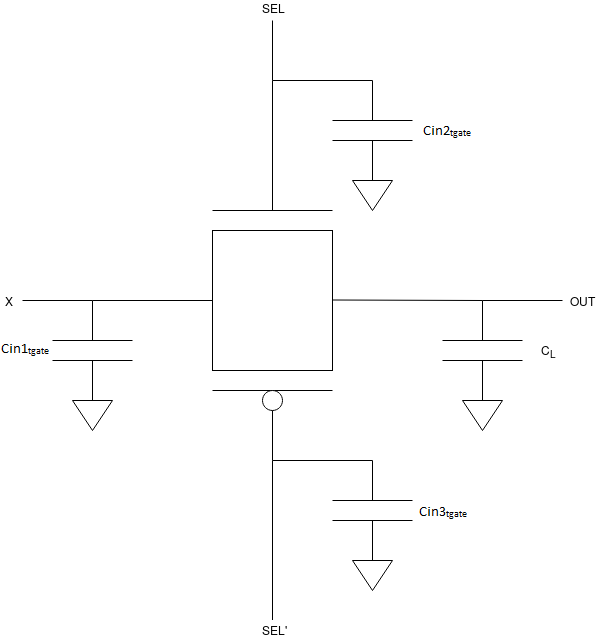
\includegraphics[width = 9 cm, height = 8 cm]{pentium/transmission_gate_interno.png}
\caption{Internal circuit of the transmission gate}
\label{tgate_interno}
\end{figure}

From Figure \ref{tgate_interno} it can be seen that the input capacitances of the transmission gate $C_{in1_{tgate}}$, $C_{in2_{tgate}}$ and $C_{in3_{tgate}}$ can be different. As said previously their values are given externally.\\
Also the area $A_{tgate}$ and the leakage current $I_{leak_{tgate}}$ are given.\\
The delay of the transmission gate is the time required for the signal at the input $X$ to reach the output node ($OUT$) when the two transistors become ON. This delay is equal to $\tau_{int_{tgate}}+\alpha_{tgate}\cdot C_L$ where $\tau_{int_{tgate}}$ and $\alpha_{tgate}$ are both given.





\subsubsection{Multiplexer 2:1}
From the transmission gate described before, a 2:1 way multiplexer (mux) can be designed and characterized. Figure \ref{fig:2to1mux} reports the designed mux.

\begin{figure}[H]
\centering
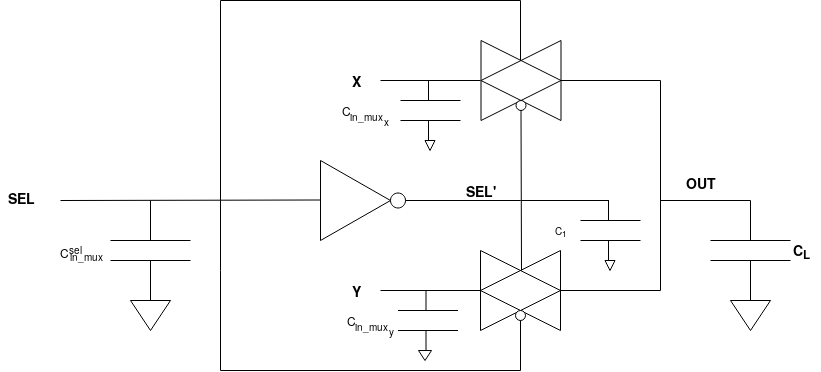
\includegraphics[width = 11.5 cm, height = 6 cm]{pentium/mux2.png}
\caption{2:1 way multiplexer implementation with transmission gates}
\label{fig:2to1mux}
\end{figure}

The black-box model used for the multiplexer is the one in figure \ref{fig:mux_black_box}.

\begin{figure}[H]
\centering
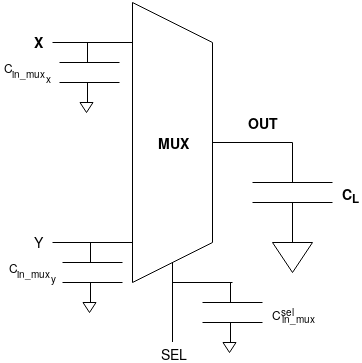
\includegraphics[width = 8 cm, height = 7 cm]{pentium/mux_schematic.png}
\caption{Multiplexer 2:1 symbol}
\label{fig:mux_black_box}
\end{figure}

%%%%%%%%%%%%%%%%%% Mux Formulas %%%%%%%%%%%%%%%%%%%%

 The multiplexer area is given by:
\begin{equation}
A_{mux} = A_{inv} + 2 A_{tgate}
\end{equation}
The leakage current is given by:
\begin{equation}
I_{leak_{mux}} = I_{leak_{inv}} + 2 I_{leak_{tgate}}
\label{eq:leak_cur_mux}
\end{equation}
The static power is
\begin{equation}
P_{stat_{mux}} = V_{DD} I_{leak_{mux}}
\end{equation}
Looking at the figure \ref{fig:2to1mux}, the dynamic power can be derived:
\begin{equation}
P_{dyn_{mux}} = V_{DD}^2 f_{CLK} E_{sw} C_1 
\end{equation}
Since $C_1 = C_{in2_{tgate}} + C_{in3_{tgate}}$ it is possible to obtain:
\begin{equation}
P_{dyn_{mux}} =  V_{DD}^2 f_{CLK} E_{sw}  (C_{in2_{tgate}} + C_{in3_{tgate}})
\end{equation}
The intrinsic delay (the delay without load) for the mux is:
\begin{equation}
\tau_{int_{mux}} = \tau_{int_{inv}} + \alpha_{inv} C_1 +\tau_{int_{tgate}}
\end{equation}
Replacing $C_1$
\begin{equation}
\tau_{int_{mux}} = \tau_{int_{inv}} + \alpha_{inv} (C_{in2_{tgate}} + C_{in3_{tgate}}) + \tau_{int_{tgate}}
\end{equation}

The $\alpha$ coefficient is:
\begin{equation}
\alpha_{mux} = \alpha_{tgate}
\end{equation}
Thus the overall delay is $\tau_{int_{mux}} + \alpha_{mux} C_L$. The input capacitance seen from the inputs X or Y is given by:
\begin{equation}
C_{in_{mux}}^{input} = C_{in_{mux_x}} = C_{in_{mux_y}} = C_{in1_{tgate}} 
\end{equation}
while the input capacitance seen from the select input is:
\begin{equation}
C_{in_{mux}}^{sel} = C_{in_{inv}} + C_{in2_{tgate}} + C_{in3_{tgate}}
\end{equation}





\subsubsection{Multiplexer 2:1 for M-length signal vectors}
In the Pentium IV adder design is useful a compact rappresentation of a selector which takes two vectors with a length equal to M and takes one of them to the output. Figure \ref{fig:M_sig_length_2to1mux} shows the implementation of such mux (called for brevity M-mux), while figure \ref{fig:mux_black_box_m} reports the black-box symbol.

\begin{figure}[H]
\centering
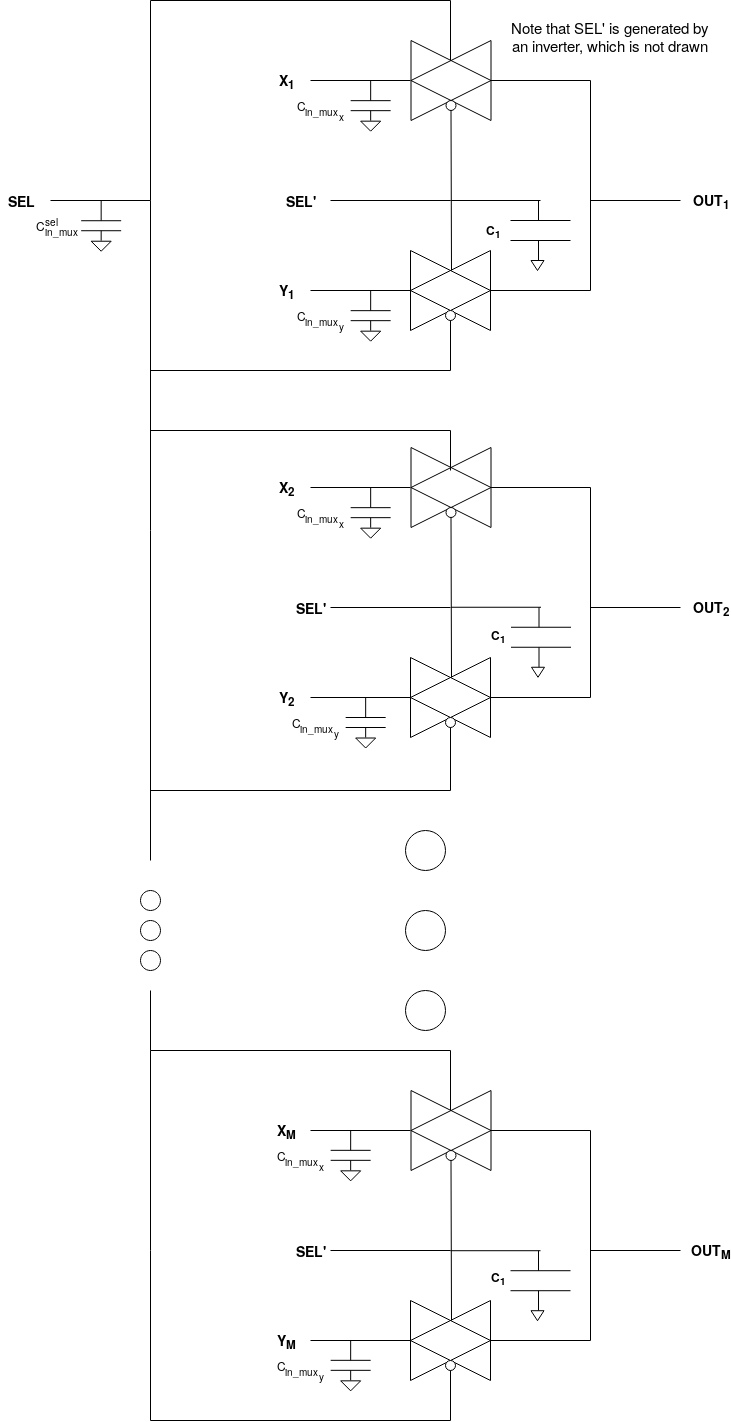
\includegraphics[width = 8 cm, height = 14 cm]{pentium/four_2to1_mux.png}
\caption{Mux 2:1 with M-bit inputs}
%\caption{implementation of a M-signal-length 2 to 1 mux}
\label{fig:M_sig_length_2to1mux}
\end{figure}

\begin{figure}[H]
\centering
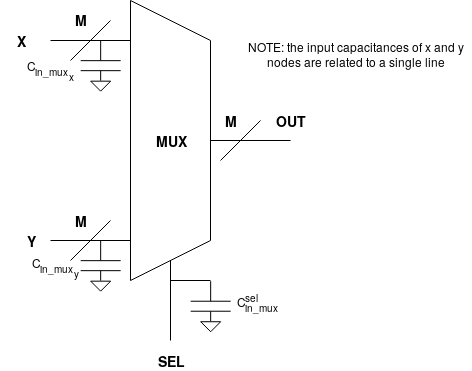
\includegraphics[width = 8 cm, height = 6 cm]{pentium/mux_schematic_m.png}
%\caption{mux for m-length signal block symbol}
\caption{Symbol of mux 2:1 with M-bit inputs}
\label{fig:mux_black_box_m} 
\end{figure}

%%%%%%%%%%%%%%%%%%%%%%%%%%%%%%%%%%%%%%%%%%%%%%%%%%%
%% Generalized mux formulas
%%%%%%%%%%%%%%%%%%%%%%%%%%%%%%%%%%%%%%%%%%%%%%%%%%%
Since in figure \ref{fig:M_sig_length_2to1mux} the SEL' signal is generated by an inverter which is not drawn, the area of the M-mux is:
\begin{equation}
A_{M-mux} = A_{inv} + 2M A_{tgate}
\end{equation}

The leakage current is given by:
\begin{equation}
I_{leak_{M-mux}} = I_{leak_{inv}} + 2M I_{leak_{tgate}}
\end{equation}

The static power is given by:
\begin{equation}
P_{stat_{M-mux}} = V_{DD} I_{leak_{M-mux}}
\end{equation}

The dynamic power is given by:
\begin{equation}
P_{dyn_{M-mux}} = V_{DD}^2 f_{CLK} E_{sw} \cdot M (C_{in2_{tgate}} + C_{in3_{tgate}})
\end{equation}

The intrinsic delay is:
\begin{equation}
\tau_{int_{M-mux}} = \tau_{int_{inv}} + \alpha_{inv} M (C_{in2_{tgate}} + C_{in3_{tgate}}) + \tau_{int_{tgate}}
\end{equation}

The $\alpha$ coefficient for the M-mux is: 
\begin{equation}
\alpha_{M-mux} = \alpha_{tgate}
\end{equation}

%Figure \ref{fig:m_2to1_mux_capacitance_schematic} shows the equivalent capacitances which has to be taken into account when the m-mux is used with reference to the 2 to 1 mux.

%\begin{figure}[H]
%\centering
%\includegraphics[width = 9 cm, height = 3 cm]{m_2to1_mux_capacitance_schematics.png}
%\caption{m-mux equivalent circuit for capacitance calculation.}
%\label{fig:m_2to1_mux_capacitance_schematic}
%\end{figure}

The input capacitances for each line of the x and y inputs are:
\begin{equation}
C_{in_{M-mux}}^{input} = C_{in_{mux_x}} = C_{in_{mux_y}} = C_{in1_{tgate}} 
\end{equation}
while the input capacitance seen from the select input is:
\begin{equation}
C_{in_{M-mux}}^{sel} = C_{in_{inv}} + M( C_{in2_{tgate}} + C_{in3_{tgate}})
\end{equation}





\subsubsection{Carry-select block}
The schematic of the carry-select block and its corresponding black box are reported in Figure \ref{fig:carry_select_schematic_bb}.

\begin{figure}[H]
\centering
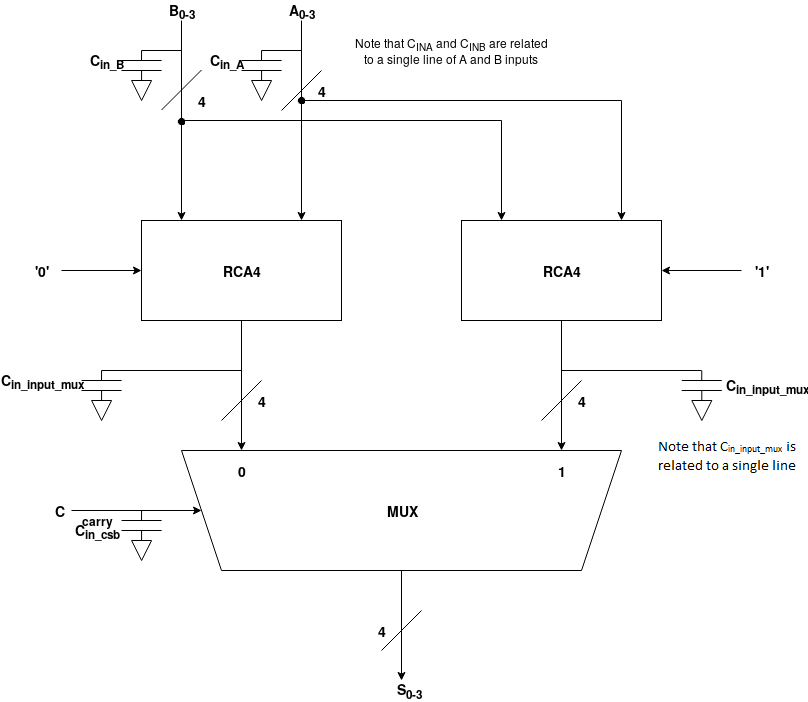
\includegraphics[width = 6 cm, height = 7 cm]{pentium/carry_select_adder_schematic.png}
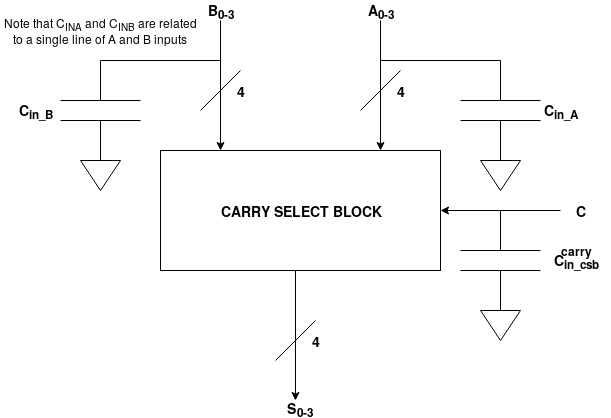
\includegraphics[width = 6 cm, height = 7 cm]{pentium/carry_select_adder_black_box.png} 
\caption{Carry-select block schematic view and block symbol}
\label{fig:carry_select_schematic_bb}
\end{figure}

The area of the carry-select block is given by:
\begin{equation}
A_{csb} = 2A_{RCA4} + A_{4-mux} 
\end{equation}

The leakage current is:
\begin{equation}
I_{leak_{csb}} = 2I_{leak_{RCA4}} + I_{leak_{4-mux}}
\end{equation}

The static power is given by:
\begin{equation}
P_{stat_{csb}} = V_{DD} I_{leak_{csb}} 
\end{equation}

The dynamic power is given by:
\begin{equation}
P_{dyn_{csb}} = V_{DD}^2 f_{CLK} E_{sw} (8 C_{in_{4-mux}}^{input}) + 2P_{dyn_{RCA4}} + P_{dyn_{4-mux}}
\end{equation}

Assuming that all the inputs $A_{0-3}$, $B_{0-3}$ and $C$ are stable, the delay is that of the path from $A_{0-3}$ and $B_{0-3}$ to $S_{0-3}$. Therefore the intrinsic delay (the delay without load) is:
\begin{equation}
\tau_{int_{csb}} = \tau_{int_{RCA4}} + \alpha_{RCA4} C_{in_{4-mux}}^{input} + \tau_{int_{4-mux}}
\end{equation}
The $\alpha$ coefficient of the carry-select block is:
\begin{equation}
\alpha_{csb} = \alpha_{4-mux}
\end{equation}

The input capacitance of a single input line ($A_{0-3}$ or $B_{0-3}$) is:
\begin{equation}
C_{in_{csb}}^{input} = C_{in_B} = C_{in_A} = 2 C_{in_{RCA4}}
\end{equation}
The carry input capacitance of the carry-select block is
\begin{equation}
C_{in_{csb}}^{carry} = C_{in_{4-mux}}^{sel}
\end{equation}





\subsubsection{Carry-select sum generator}
Carry-select sum generator (cssg) schematic is reported in figure \ref{fig:cssg_schematic} and its black box symbol in figure \ref{fig:cssg_bb}. In these figures the number of bits is set to 32.

\begin{figure}[H]
\centering
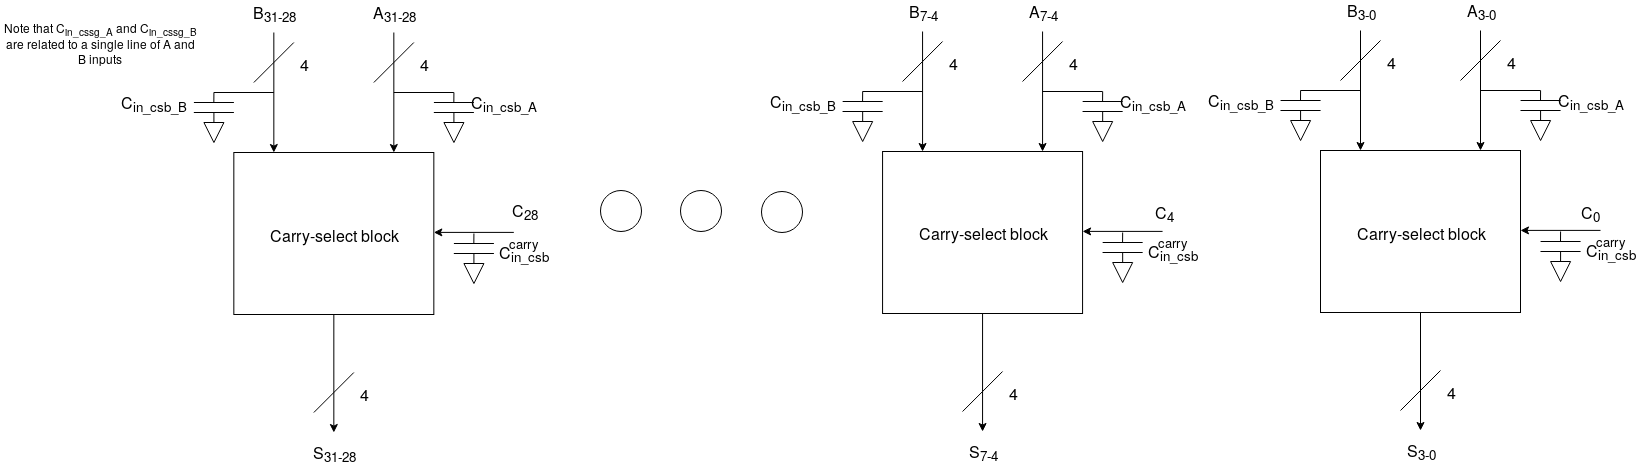
\includegraphics[width = 14 cm, height = 6 cm]{pentium/carry_select_sum_generator_schematic.png}
\caption{Carry-select sum generator schematic}
\label{fig:cssg_schematic}
\end{figure}

\begin{figure}[H]
\centering
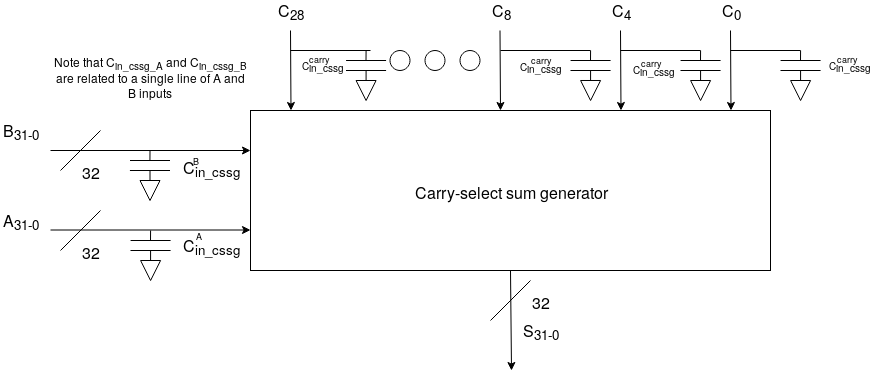
\includegraphics[width = 10 cm, height = 6 cm]{pentium/carry_select_sum_generator_black_box.png}
\caption{Carry-select sum generator black-box}
\label{fig:cssg_bb}
\end{figure}

Introducing $N$, which is the number of bits of the adder, the area can be derived:

\begin{equation}
A_{cssg} = \frac{N}{4} A_{csb}
\end{equation}

Note that the values of $N$ considered are 8, 12, 16, 20, 24, 28 and 32.

The leakage current is:
\begin{equation}
I_{leak_{cssg}} = \frac{N}{4} I_{leak_{csb}}
\end{equation}

The static power is:

\begin{equation}
P_{stat_{cssg}} = V_{DD} I_{leak_{cssg}}
\end{equation}

The dynamic power is:

\begin{equation}
P_{dyn_{cssg}} = \frac{N}{4} P_{dyn_{csb}}
\end{equation}

The intrinsic delay (the delay without load) is:
\begin{equation}
\tau_{int_{cssg}} = \tau_{int_{csb}}
\end{equation}

The $\alpha$ parameter is:
\begin{equation}
\alpha_{cssg} = \alpha_{csb}
\end{equation}

The input capacitances for each line of the A and B inputs are:
\begin{equation}
C_{in_{cssg}}^{input} = C_{in_{cssg}}^{A} = C_{in_{cssg}}^{B} = C_{in_{csb}}^{input}
\end{equation}
while the input capacitance seen from each carry input is:

\begin{equation}
C_{in_{cssg}}^{carry} = C_{in_{csb}}^{carry}
\end{equation}





\subsection{Carry-merge sparse tree}
In this subsection the three blocks that constitute the carry-merge sparse tree are presented. They are the pre-computation block (pcb), the propagate-generate block (pg) and the G-block (gb). Using these blocks the carry-merge sparse tree can be designed.





\subsubsection{Pre-computation block}
In figure \ref{pcb} it is shown the symbol and the schematic view of the pre-computation block.

\begin{figure}[H]
\centering
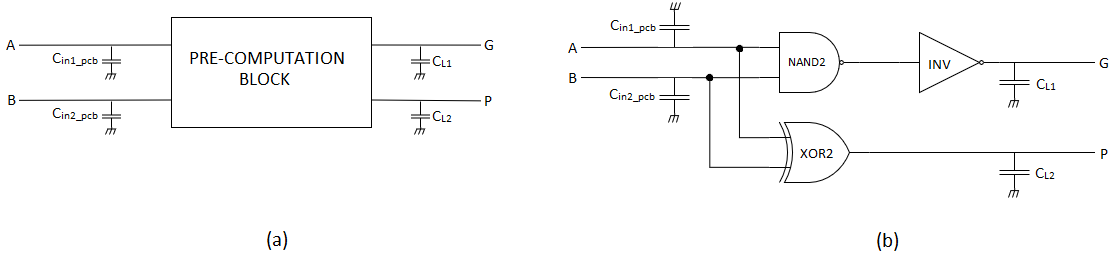
\includegraphics[width = 14cm]{pentium/pcb.png}
\caption{Pre-computation block. (a) Symbol. (b) Schematic view. }
\label{pcb}
\end{figure}

The  area of the pre-computation block is given by:
\begin{equation}
A_{pcb}=A_{nand2}+A_{inv}+A_{xor2}
\end{equation}
The leakage current is:
\begin{equation}
I_{leak_{pcb}}=I_{leak_{nand2}}+I_{leak_{inv}}+I_{leak_{xor2}}
\end{equation}
The static power is:
\begin{equation}
P_{stat_{pcb}}=V_{DD}\cdot I_{leak_{pcb}}
\end{equation}
The dynamic power is:
\begin{equation}
P_{dyn_{pcb}}=V_{DD}^2f_{CLK}E_{sw}C_{in_{inv}}
\end{equation}

The intrinsic delay (the delay without load) of the output $G$ is:
\begin{equation}
\tau_{int_{pcb_{G}}} = \tau_{int_{nand2}}+\alpha_{nand2}C_{in_{inv}}+\tau_{int_{inv}}
\end{equation}

Then the $\alpha$ parameter is:
\begin{equation}
\alpha_{pcb_{G}}=\alpha_{inv}
\end{equation}

Thus the total delay of $G$ (considering the load) is $\tau_{int_{pcb_{G}}}+\alpha_{pcb_{G}}C_{L1}$.\\\\

Analogously for the output $P$ we have:
\begin{equation}
\tau_{int_{pcb_{P}}} = \tau_{int_{xor2}}
\end{equation}

\begin{equation}
\alpha_{pcb_{P}}=\alpha_{xor2}
\end{equation}

The delay of $P$ considering the load will be $\tau_{int_{pcb_{P}}}+\alpha_{pcb_{P}}C_{L2}$.\\\\

The input capacitances of the pre-computation block are:
\begin{equation}
C_{in_{pcb}}=C_{in1_{pcb}}=C_{in2_{pcb}}=C_{in_{nand2}}+C_{in_{xor2}}
\end{equation}





\subsubsection{Propagate-generate block}
Figure \ref{fig:pg_block_schematic} shows the propagate-generate block (pg-block) schematic and figure \ref{fig:pg_bb} its black-box model.

\begin{figure}[H]
\centering
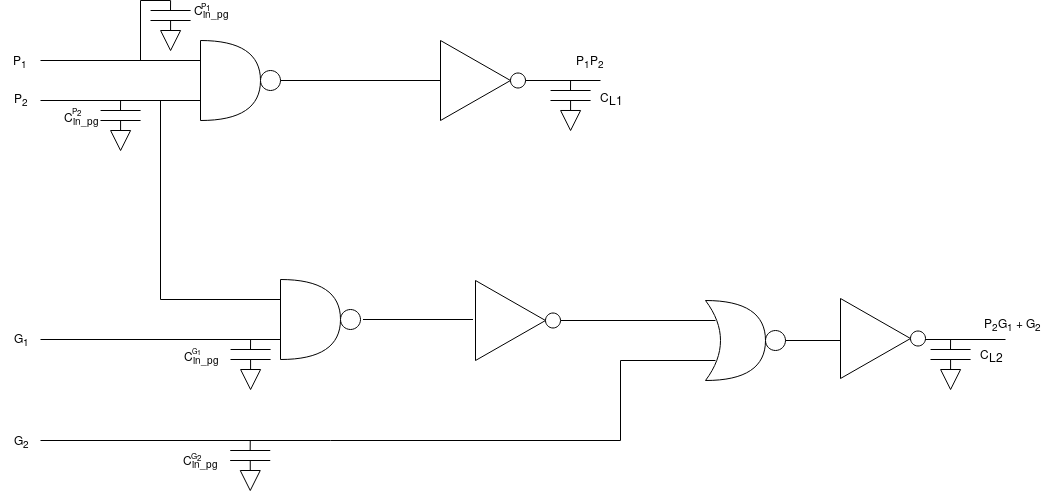
\includegraphics[width = \textwidth]{pentium/propagate_generate_block_schematic.png}
\caption{Schematic of propagate and generate carry block}
\label{fig:pg_block_schematic}
\end{figure}

\begin{figure}[H]
\centering
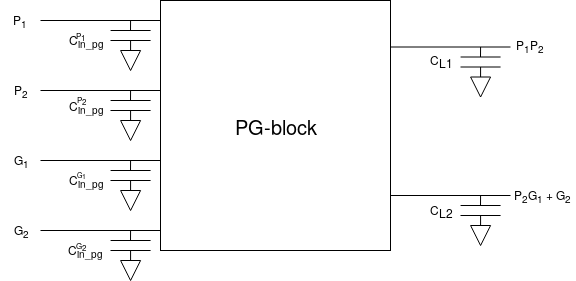
\includegraphics[width = 8 cm]{pentium/propagate_generate_block_black_box.png}
\caption{Symbol of propagate and generate carry block}
\label{fig:pg_bb}
\end{figure}

From the schematic figure, the area can be evaluated as:
\begin{equation}
A_{pg} = 2 A_{nand2} + A_{nor2} + 3 A_{inv}
\end{equation}

The leakage current is:
\begin{equation}
I_{leak_{pg}} = 2 I_{leak_{nand2}} + I_{leak_{nor2}} + 3 I_{leak_{inv}}
\end{equation}

The static power is:
\begin{equation}
P_{stat_{pg}} = V_{DD} I_{leak_{pg}}
\end{equation}

The dynamic power is:
\begin{equation}
P_{dyn_{pg}} = V_{DD}^2 f_{CLK} E_{sw} (3 C_{in_{inv}}  +  C_{in_{nor2}})
\end{equation}

The intrinsic delay (delay without load) for the $P_1 P_2$ output is:
\begin{equation}
\tau_{int_{pg_p}} = \tau_{int_{nand2}} + \alpha_{nand2} C_{in_{inv}} + \tau_{int_{inv}}
\end{equation}
The $\alpha$ parameter is:
\begin{equation}
\alpha_{pg_p} = \alpha_{inv}
\end{equation}
Thus the overall delay for the $P_1 P_2$ output  is $\tau_{int_{pg_p}} + \alpha_{pg_p} C_{L1}$.\\


The intrinsic delay for the $P_2G_1+G_2$  output is:
\begin{equation}
\tau_{int_{pg_g}} = \tau_{int_{nand2}} + \alpha_{nand2} C_{in_{inv}} + \tau_{int_{inv}} + \alpha_{inv} C_{in_{nor2}} + \tau_{int_{nor2}} + \alpha_{nor2} C_{in_{inv}} + \tau_{int_{inv}}
\end{equation}
The $\alpha$ parameter is:
\begin{equation}
\alpha_{pg_g} = \alpha_{inv}
\end{equation}
The overall delay of this output is $ \tau_{int_{pg_g}} + \alpha_{pg_g} C_{L2}$.\\

In order from $P_1$ to $G_2$, the input capacitances are:
\begin{equation}
C_{in_{pg}}^{P_1} = C_{in_{nand2}}
\end{equation}

\begin{equation}
C_{in_{pg}}^{P_2} = 2 C_{in_{nand2}}
\end{equation}

\begin{equation}
C_{in_{pg}}^{G_1} = C_{in_{nand2}}
\end{equation}

\begin{equation}
C_{in_{pg}}^{G_2} = C_{in_{nor2}}
\end{equation}

Then the total input capacitance for this block is defined as:
\begin{equation}
C_{in_{pg}}^{tot} = C_{in_{pg}}^{P_1} + C_{in_{pg}}^{P_2} + C_{in_{pg}}^{G_1} + C_{in_{pg}}^{G_2}
\end{equation}





\subsubsection{G-block}
This block is the same of the previous one but there is only the second output (G-output). In figure \ref{gb} it is shown the symbol and the schematic view of the G-block.

\begin{figure}[H]
\centering
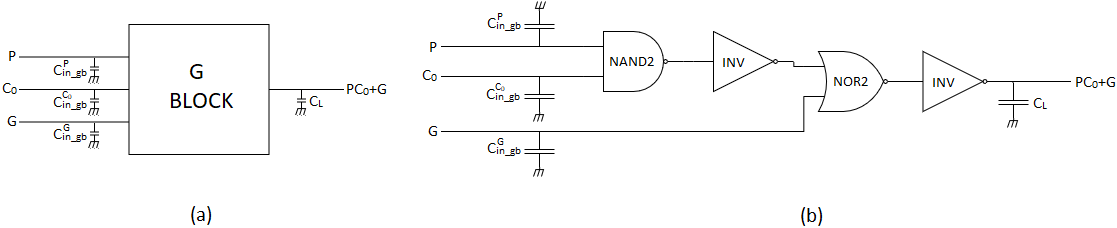
\includegraphics[width = 14cm]{pentium/gb.png}
\caption{G-block. (a) Symbol. (b) Schematic view. }
\label{gb}
\end{figure}

The  area of the G-block is given by:
\begin{equation}
A_{gb}=A_{nand2}+A_{nor2}+2A_{inv}
\end{equation}
The leakage current is:
\begin{equation}
I_{leak_{gb}}=I_{leak_{nand2}}+I_{leak_{nor2}}+2I_{leak_{inv}}
\end{equation}
The static power is:
\begin{equation}
P_{stat_{gb}}=V_{DD}\cdot I_{leak_{gb}}
\end{equation}
The dynamic power is:
\begin{equation}
P_{dyn_{gb}}=V_{DD}^2f_{CLK}E_{sw}(2C_{in_{inv}}+C_{in_{nor2}})
\end{equation}

The intrinsic delay (the delay without load) is:
\begin{equation}
\tau_{int_{gb}} = \tau_{int_{nand2}} + \alpha_{nand2} C_{in_{inv}} + \tau_{int_{inv}} + \alpha_{inv} C_{in_{nor2}} + \tau_{int_{nor2}} + \alpha_{nor2} C_{in_{inv}} + \tau_{int_{inv}}
\end{equation}

Then the $\alpha$ parameter is:
\begin{equation}
\alpha_{gb}=\alpha_{inv}
\end{equation}

Thus the total delay (considering the load) is $\tau_{int_{gb}}+\alpha_{gb}C_{L}$.\\\\
The input capacitances are:
\begin{equation}
C_{in_{gb}}^{P} = C_{in_{nand2}}
\end{equation}
\begin{equation}
C_{in_{gb}}^{C_0} = C_{in_{nand2}}
\end{equation}
\begin{equation}
C_{in_{gb}}^{G} = C_{in_{nor2}}
\end{equation}





\subsubsection{Carry-merge sparse tree}
In Figure \ref{tree_black_box} and in Figure \ref{tree_interno} are respectively shown the black-box and the schematic view of the carry-merge sparse tree for a number of bit $N=32$.

\begin{figure}[H]
\centering
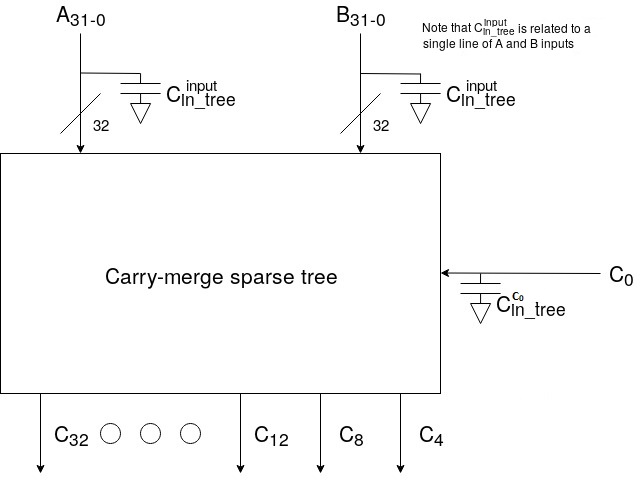
\includegraphics[width = 8cm]{pentium/tree_black_box.jpeg}
\caption{Symbol of carry-merge sparse tree with 32 bit}
\label{tree_black_box}
\end{figure}

\begin{figure}[H]
\centering
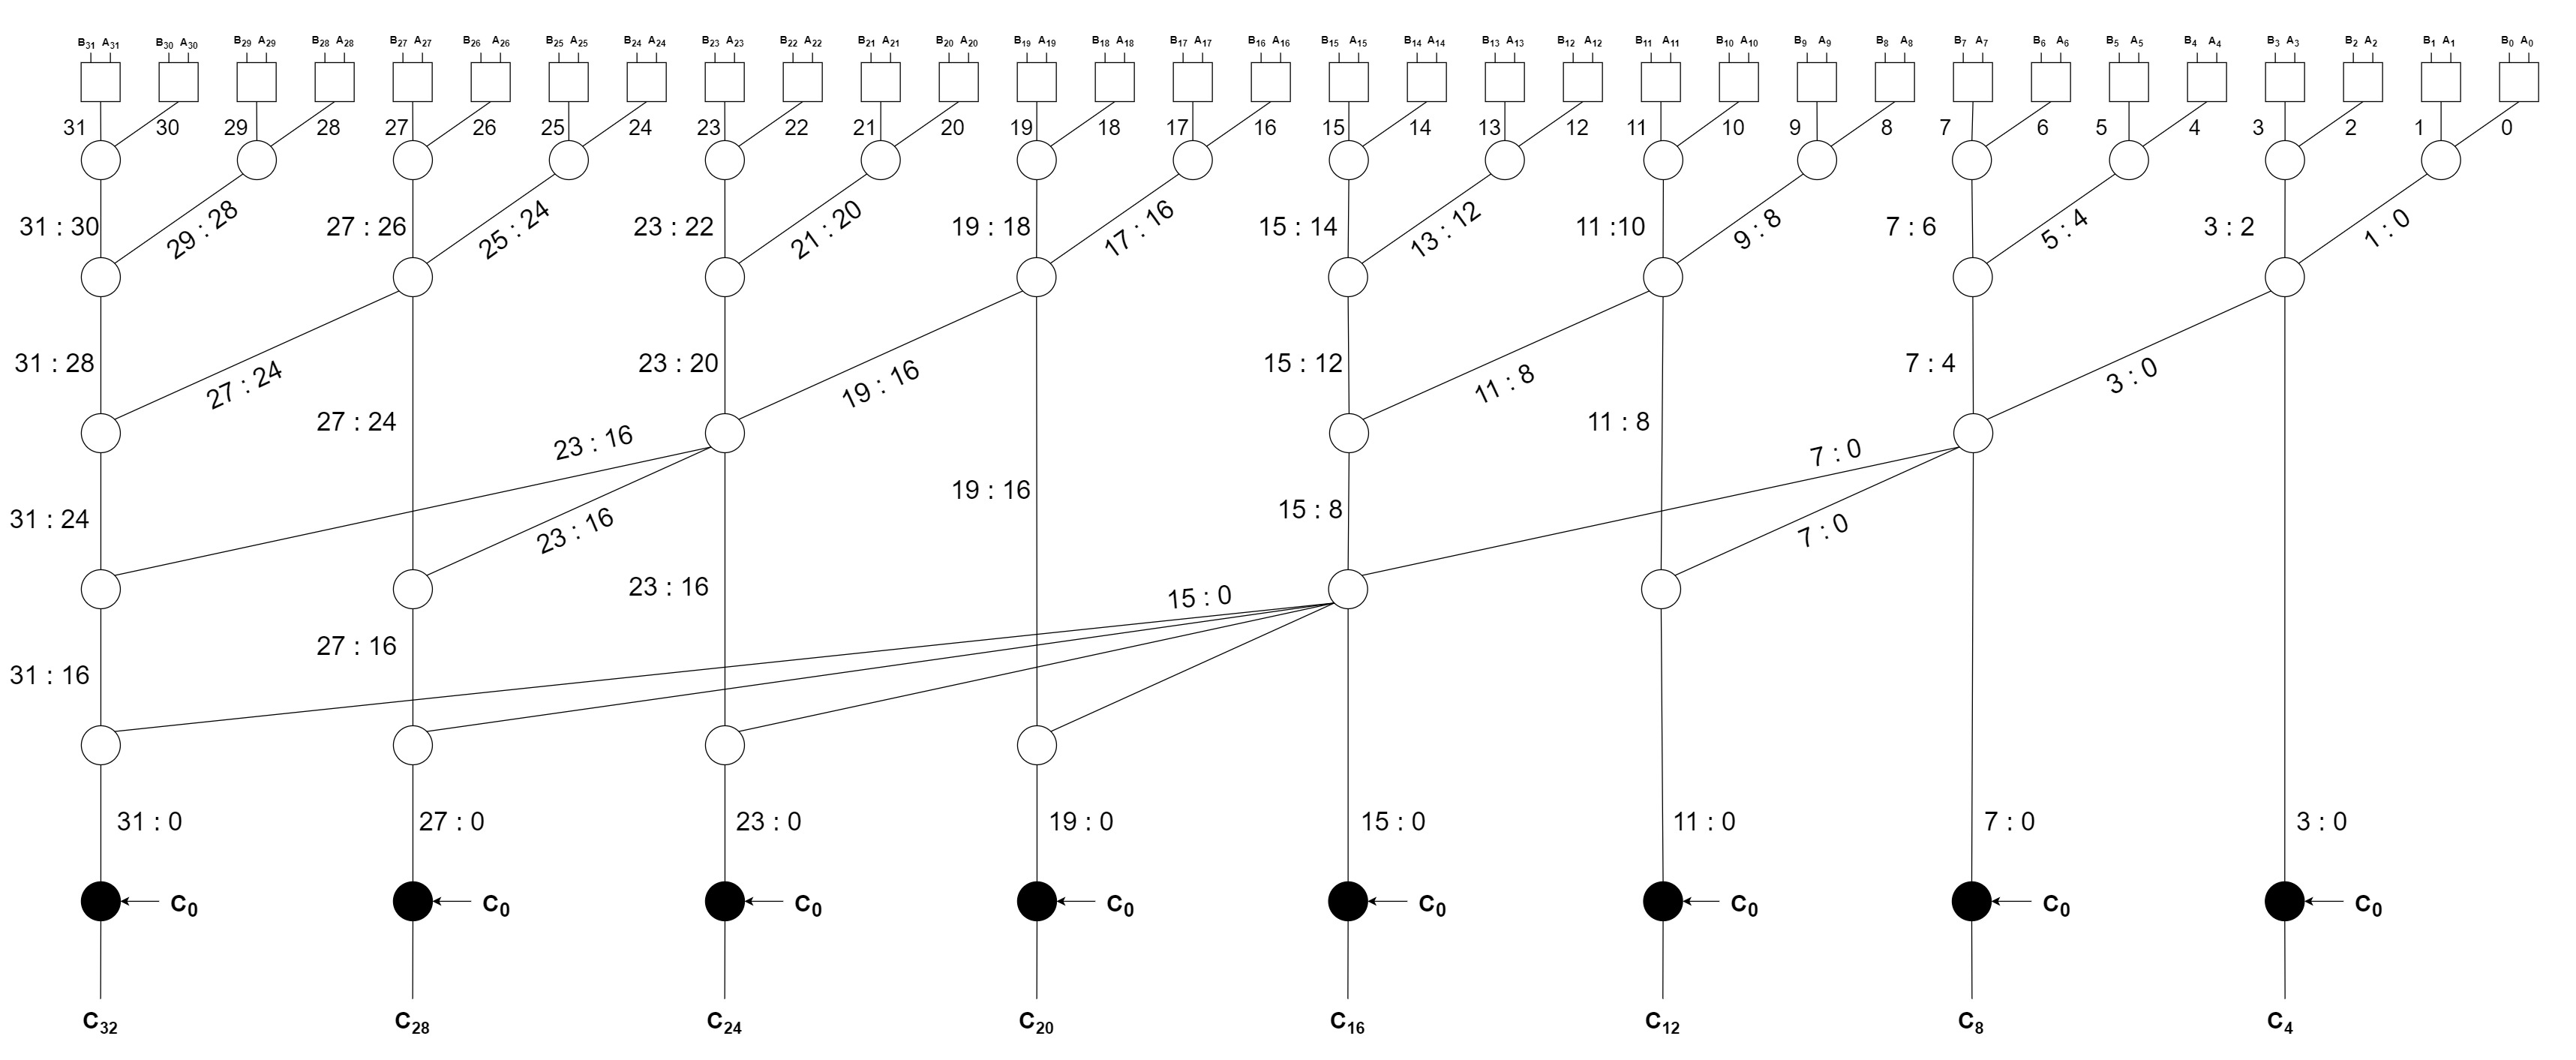
\includegraphics[width = 14cm]{pentium/tree_interno.jpg}
\caption{Schematic view of the carry-merge sparse tree with 32 bit}
\label{tree_interno}
\end{figure}

In the schematic view the white squares are pre-computation blocks (pcb), the white circles are propagate-generate blocks (pg) and the black circles are G-blocks (gb). Note that the pcb and pg-blocks have two output but in the schematic view there is only one line for both of them. This is only to have a less complicated picture of the schematic view.\\
The outputs of this tree are the carry from $C_4$ to $C_{32}$ with a step of 4.\\
Area, power consumption and delay of the tree are evaluated as a function of the number of bit $N$, in the case where $N$ can be equal to 8, 12, 16, 20, 24, 28 or 32.\\
The area of the tree is equal to:
\begin{equation}
A_{tree} = N_{pcb}A_{pcb}+N_{pg}A_{pg}+N_{gb}A_{gb}
\end{equation}

Where:
\begin{equation}
N_{pcb}=N
\end{equation}
and
\begin{equation}
N_{gb}=\frac{N}{4}
\end{equation}
$N_{pg}$ cannot be written as a function of $N$ in a simple way. Therefore the number of pg-blocks for each case looking at the figure \ref{tree_interno} can be counted.
\begin{equation}
N_{pg}=
   \begin{cases}
   7 \,\,\,\,\,\,\,\,\,\,\,\,\,\, N=8 \\
   11 \,\,\,\,\,\,\,\,\,\,\, N=12 \\
   16 \,\,\,\,\,\,\,\,\,\,\, N=16 \\
   20 \,\,\,\,\,\,\,\,\,\,\, N=20 \\
   25 \,\,\,\,\,\,\,\,\,\,\, N=24 \\
   30 \,\,\,\,\,\,\,\,\,\,\, N=28 \\
   36 \,\,\,\,\,\,\,\,\,\,\, N=32 \\
   \end{cases}
\end{equation}


The leakage current is given by:
\begin{equation}
I_{leak_{tree}}=N_{pcb}I_{leak_{pcb}}+N_{pg}I_{leak_{pg}}+N_{gb}I_{leak_{gb}}
\end{equation}
The static power is:
\begin{equation}
P_{stat_{tree}}=V_{DD}\cdot I_{leak_{tree}}
\end{equation}
The dynamic power is:
\begin{equation}
P_{dyn_{tree}} = V_{DD}^2 f_{CLK} E_{sw} \Bigl[N_{pg}C_{in_{pg}}^{tot} + N_{gb}\bigl( C_{in_{gb}}^{P}+ C_{in_{gb}}^{G} \bigr)\Bigr] + N_{pcb} P_{dyn_{pcb}} + N_{pg} P_{pyn_{pg}} + N_{gb} P_{dyn_{gb}}
\end{equation}

Without doing simplifications (for instance considering an upper bound for the delay instead of the real delay), there is not a simple way to evaluate the delay of the tree as a function of $N$. This is why when $N$ changes, the capacitances in the nodes of the tree can change.\\
To evaluate the delay of the tree no simplifications are used. For this reason, each case of $N$ is considered separately.\\\\
First of all, we note that the pcb-blocks have always the same load for each value of $N$. Thus we can compute the total delay of a pcb-block as:
\begin{equation}
\tau_{pcb_{tree}} = max\Bigl(\tau_{pcb_{tree}}^G, \tau_{pcb_{tree}}^P\Bigr)
\end{equation}
where $\tau_{pcb_{tree}}^G$ is the delay related to the $G$ output while $\tau_{pcb_{tree}}^P$ is related to the $P$ one. Since the load of each the pcb-block is always one pg-block, it can be written:
\begin{equation}
\tau_{pcb_{tree}}^G = \tau_{int_{pcb_{G}}} +  \alpha_{pcb_{G}} \cdot max\Bigl(C_{in_{pg}}^{G_1}, C_{in_{pg}}^{G_2} \Bigr)
\end{equation}
\begin{equation}
\tau_{pcb_{tree}}^P = \tau_{int_{pcb_{P}}} +  \alpha_{pcb_{P}} \cdot max\Bigl(C_{in_{pg}}^{P_1}, C_{in_{pg}}^{P_2} \Bigr)
\end{equation}

In order to compute the delay of the tree for each value of $N$, it is useful computing the delay of the pg-block for different loads. \\
$\tau_{pg_{xy}}^G$ is the delay related to the output $G$ of a pg-block  when the load is a number $x$ of pg-blocks and a number $y$ of G-blocks. Similarly $\tau_{pg_{xy}}^P$ is the delay related to the output $P$ of a pg-block  when the load is a number $x$ of pg-blocks and a number $y$ of G-blocks.\\

Thus the delay of a pg-block with a load of 1 pg-block and 0 G-block is:
\begin{equation}
\tau_{pg_{10}} = max\Bigl( \tau_{pg_{10}}^G, \tau_{pg_{10}}^P \Bigr)
\end{equation}
 where:
\begin{equation}
\tau_{pg_{10}}^G = \tau_{int_{pg_g}} + \alpha_{pg_g} \cdot max\Bigl( C_{in_{pg}}^{G_1}, C_{in_{pg}}^{G_2}  \Bigr)
\end{equation}
\begin{equation}
\tau_{pg_{10}}^P = \tau_{int_{pg_p}} + \alpha_{pg_p} \cdot max\Bigl( C_{in_{pg}}^{P_1}, C_{in_{pg}}^{P_2}  \Bigr)
\end{equation}
\\
The delay of a pg-block with a load of 1 pg-block and 1 G-block is:
\begin{equation}
\tau_{pg_{11}} = max\Bigl( \tau_{pg_{11}}^G, \tau_{pg_{11}}^P \Bigr)
\end{equation}
 where:
\begin{equation}
\tau_{pg_{11}}^G = \tau_{int_{pg_g}} + \alpha_{pg_g} \cdot \Bigl[ max\Bigl( C_{in_{pg}}^{G_1}, C_{in_{pg}}^{G_2}  \Bigr) + C_{in_{gb}}^{G} \Bigr]
\end{equation}
\begin{equation}
\tau_{pg_{11}}^P = \tau_{int_{pg_p}} + \alpha_{pg_p} \cdot \Bigl[ max\Bigl( C_{in_{pg}}^{P_1}, C_{in_{pg}}^{P_2}  \Bigr) + C_{in_{gb}}^{P} \Bigr]
\end{equation}
\\
The delay of a pg-block with a load of 2 pg-block and 1 G-block is:
\begin{equation}
\tau_{pg_{21}} = max\Bigl( \tau_{pg_{21}}^G, \tau_{pg_{21}}^P \Bigr)
\end{equation}
 where:
\begin{equation}
\tau_{pg_{21}}^G = \tau_{int_{pg_g}} + \alpha_{pg_g} \cdot \Bigl[ 2max\Bigl( C_{in_{pg}}^{G_1}, C_{in_{pg}}^{G_2}  \Bigr) + C_{in_{gb}}^{G} \Bigr]
\end{equation}
\begin{equation}
\tau_{pg_{21}}^P = \tau_{int_{pg_p}} + \alpha_{pg_p} \cdot \Bigl[ 2max\Bigl( C_{in_{pg}}^{P_1}, C_{in_{pg}}^{P_2}  \Bigr) + C_{in_{gb}}^{P} \Bigr]
\end{equation}
\\
The delay of a pg-block with a load of 4 pg-block and 1 G-block is:
\begin{equation}
\tau_{pg_{41}} = max\Bigl( \tau_{pg_{41}}^G, \tau_{pg_{41}}^P \Bigr)
\end{equation}
 where:
\begin{equation}
\tau_{pg_{41}}^G = \tau_{int_{pg_g}} + \alpha_{pg_g} \cdot \Bigl[ 4max\Bigl( C_{in_{pg}}^{G_1}, C_{in_{pg}}^{G_2}  \Bigr) + C_{in_{gb}}^{G} \Bigr]
\end{equation}
\begin{equation}
\tau_{pg_{41}}^P = \tau_{int_{pg_p}} + \alpha_{pg_p} \cdot \Bigl[ 4max\Bigl( C_{in_{pg}}^{P_1}, C_{in_{pg}}^{P_2}  \Bigr) + C_{in_{gb}}^{P} \Bigr]
\end{equation}
\\
The delay of a pg-block with a load of 0 pg-block and 1 G-block is:
\begin{equation}
\tau_{pg_{01}} = max\Bigl( \tau_{pg_{01}}^G, \tau_{pg_{01}}^P \Bigr)
\end{equation}
 where:
\begin{equation}
\tau_{pg_{01}}^G = \tau_{int_{pg_g}} + \alpha_{pg_g} \cdot C_{in_{gb}}^{G}
\end{equation}
\begin{equation}
\tau_{pg_{01}}^P = \tau_{int_{pg_p}} + \alpha_{pg_p} \cdot C_{in_{gb}}^{P}
\end{equation}
\\
Now the intrinsic delay (the delay without load) of the tree, for each value of $N$, can be evaluated. We will denote the intrinsic delay as $\tau_{int_{tree}}^N$ where $N$ is the number of bit. Looking at the figure \ref{tree_interno} we can write:

\begin{equation}
\tau_{int_{tree}}^{8} = \tau_{pcb_{tree}} + \tau_{pg_{10}} + \tau_{pg_{11}} + \tau_{pg_{01}} + \tau_{int_{gb}}
\end{equation}
\begin{equation}
\tau_{int_{tree}}^{12} =  \tau_{pcb_{tree}} + \tau_{pg_{10}} + \tau_{pg_{11}} + \tau_{pg_{21}} + \tau_{pg_{01}} + \tau_{int_{gb}}
\end{equation}

\begin{equation}
\tau_{int_{tree}}^{16} = \tau_{int_{tree}}^{12}
\label{yeah1}
\end{equation}

\begin{equation}
\tau_{int_{tree}}^{20} = \tau_{pcb_{tree}} + \tau_{pg_{10}} + \tau_{pg_{11}} + \tau_{pg_{21}} + \tau_{pg_{41}} + \tau_{int_{gb}}
\end{equation}

\begin{equation}
\tau_{int_{tree}}^{24} = \tau_{int_{tree}}^{28} = \tau_{int_{tree}}^{32} = \tau_{int_{tree}}^{20}
\label{yeah2}
\end{equation}

The $\alpha$ coefficient of the tree does not depend on $N$ and it is equal to:
\begin{equation}
\alpha_{tree} = \alpha_{gb}
\end{equation}

The input capacitance for each line of the $A_{31-0}$ and $B_{31-0}$ inputs is:
\begin{equation}
C_{in_{tree}}^{input} = C_{in_{pcb}}
\end{equation}
while the input capacitance seen from the $C_0$:
\begin{equation}
C_{in_{tree}}^{C_0} = N_{gb}C_{in_{gb}}^{C_0}
\end{equation}





\subsection{Pentium IV adder}
The overall architecture can be summarized into the schematic in figure \ref{fig:pentium32adder_schematic}. The black-box symbol is reported in figure \ref{fig:pentium32adder_bb}.

\begin{figure}[H]
\centering
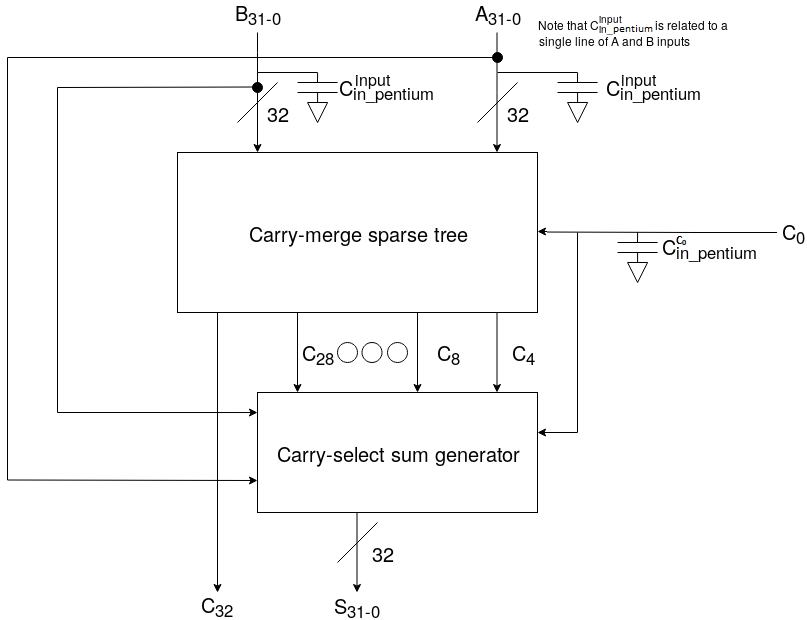
\includegraphics[width = 10 cm]{pentium/pentium32schematic.png}
\caption{Schematic of the 32-bit Pentium IV adder}
\label{fig:pentium32adder_schematic}
\end{figure}

\begin{figure}[H]
\centering
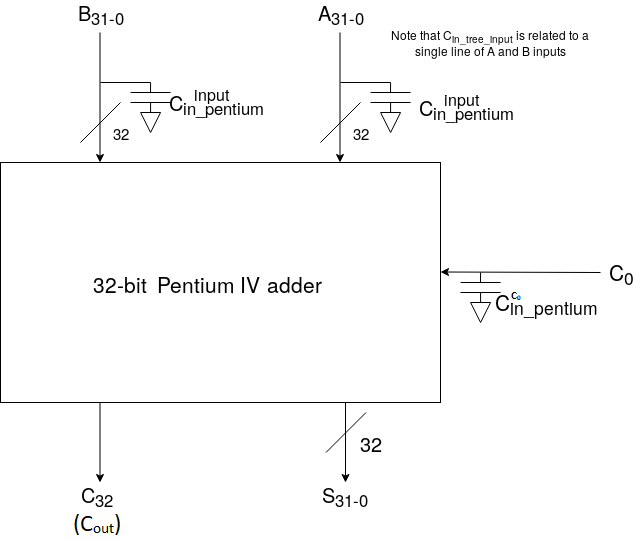
\includegraphics[width = 8 cm]{pentium/pentium32black_box.png}
\caption{Pentium IV black-box view}
\label{fig:pentium32adder_bb}
\end{figure}

The area can be evaluated as:
\begin{equation}
A_{pentium} = A_{tree} + A_{cssg}
\end{equation}

The leakage current is:
\begin{equation}
I_{leak_{pentium}} = I_{leak_{tree}} + I_{leak_{cssg}}
\end{equation}

The static power is:
\begin{equation}
P_{stat_{pentium}} = V_{DD} I_{leak_{pentium}}
\end{equation}

The dynamic power is:
\begin{equation}
P_{dyn_{pentium}} = V_{DD}^2 f_{CLK} E_{sw} \Biggl(\frac{N}{4} - 1\Biggr)C_{in_{cssg}}^{carry} + P_{dyn_{tree}} + P_{dyn_{cssg}}
\end{equation}

The input signals $A_{31-0}$ and $B_{31-0}$ enter both in the tree and in the carry-select sum generator. Thus the tree and all RCA4s inside the carry-select sum generator work in parallel. This means that if the delay of the tree ($\tau_{int_{tree}}^{N}+\alpha_{tree}C_{in_{cssg}}^{carry}$) is greater than the delay of the RCA4 ($\tau_{int_{RCA4}} + \alpha_{RCA4} C_{in_{4-mux}}^{input}$), the delay of the Pentium without load will be $\tau_{int_{tree}}^{N}+\alpha_{tree}C_{in_{cssg}}^{carry}+\tau_{int_{4-mux}}$ where $C_{in_{cssg}}^{carry} = C_{in_{csb}}^{carry}$. On the contrary, if the delay of the tree is smaller than the delay of the RCA4 (usually this case does not happen if the number of bit is big), the delay of the the Pentium without load will be $\tau_{int_{cssg}} = \tau_{int_{csb}} = \tau_{int_{RCA4}} + \alpha_{RCA4} C_{in_{4-mux}}^{input} + \tau_{int_{4-mux}}$.\\\\
Therefore the delay of the Pentium without is:
\begin{equation}
\tau_{int_{pentium}} = max \Bigl( \tau_{int_{tree}}^{N} + \alpha_{tree} C_{in_{cssg}}^{carry} + \tau_{int_{4-mux}}, \tau_{int_{cssg}} \Bigr)
\end{equation}

The $\alpha$ parameter is:
\begin{equation}
\alpha_{pentium} = \alpha_{cssg}
\end{equation}

The input capacitance for each line of the $A_{31-0}$ and $B_{31-0}$ inputs is:
\begin{equation}
C_{in_{pentium}}^{input} = C_{in_{tree}}^{input} + C_{in_{cssg}}^{input}
\end{equation}
while the input capacitance seen from the $C_0$:
\begin{equation}
C_{in_{pentium}}^{C_0} = C_{in_{tree}}^{C_0} + C_{in_{cssg}}^{carry}
\end{equation}
\\
Now the working frequency can be estimated. As already said in section \ref{ciao}, the inverse of the delay of the Pentium IV without load is used as working frequency.\\
\begin{equation}
f_{CLK} = \frac{1}{\tau_{int_{pentium}}}
\end{equation}





\section{Matlab implementation}
All the formulas in this report have been implemented in Matlab in order to evaluate area, power consumption and delay of the Pentium IV adder. Obviously the values of the input parameters described in Table \ref{library_logic_gates} are set to see the results, but  the characterization these logic gates is assumed already done by other works. For this reason reasonable values for the input parameters, considering the internal structure of the logic CMOS gates, have been used.\\
In the following is reported the Matlab code.

\lstinputlisting{pentium/Pentium_IV2.m}





\section{Results}
In this section are reported in graphs the results obtained for area, power and delay of the Pentium IV considering 8, 12, 16, 20, 24, 28 and 32 bits parallelism.\\
As expected the area increases by increasing the number of bits (figure \ref{result_area}). The static power increases with the same trend of the area (figure \ref{result_Pstat}). This is why each block in the Pentium IV has a leakage current, thus if the area increases also the static power increases.\\
If the area increases ($N$ increases), it is expected also that the dynamic power increases as it can be seen in figure \ref{result_Pdyn}.\\
Figure \ref{result_delay} shows the delay without load of the Pentium IV. It is possible to notice how the delay follows instead a different trend: this can be explained remembering that for $N=12$ and $N=16$ the tree has the exact same delay (eq.\ref{yeah1}). The same happens also in the cases in which $N=20$, $N=24$, $N=28$ and $N=32$ (eq.\ref{yeah2}).





\begin{figure}[H]
\centering
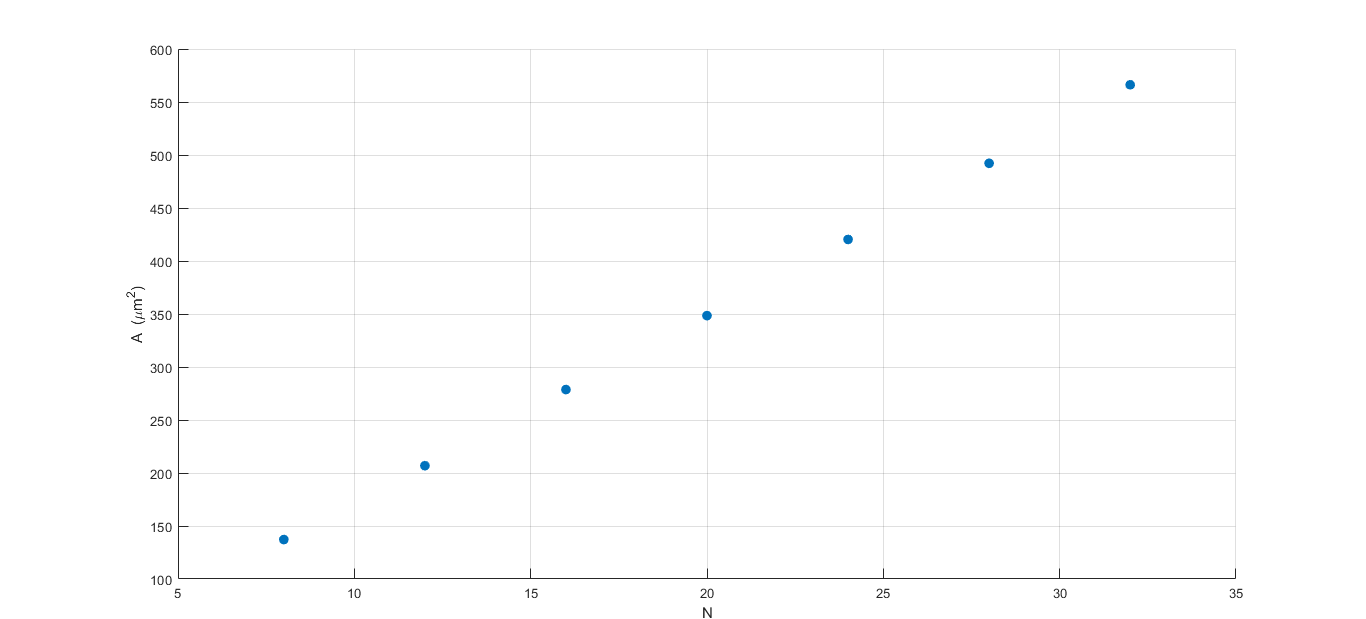
\includegraphics[width = 14 cm]{pentium/result_area.png}
\caption{Area Pentium IV as a function of $N$}
\label{result_area}
\end{figure}

\begin{figure}[H]
\centering
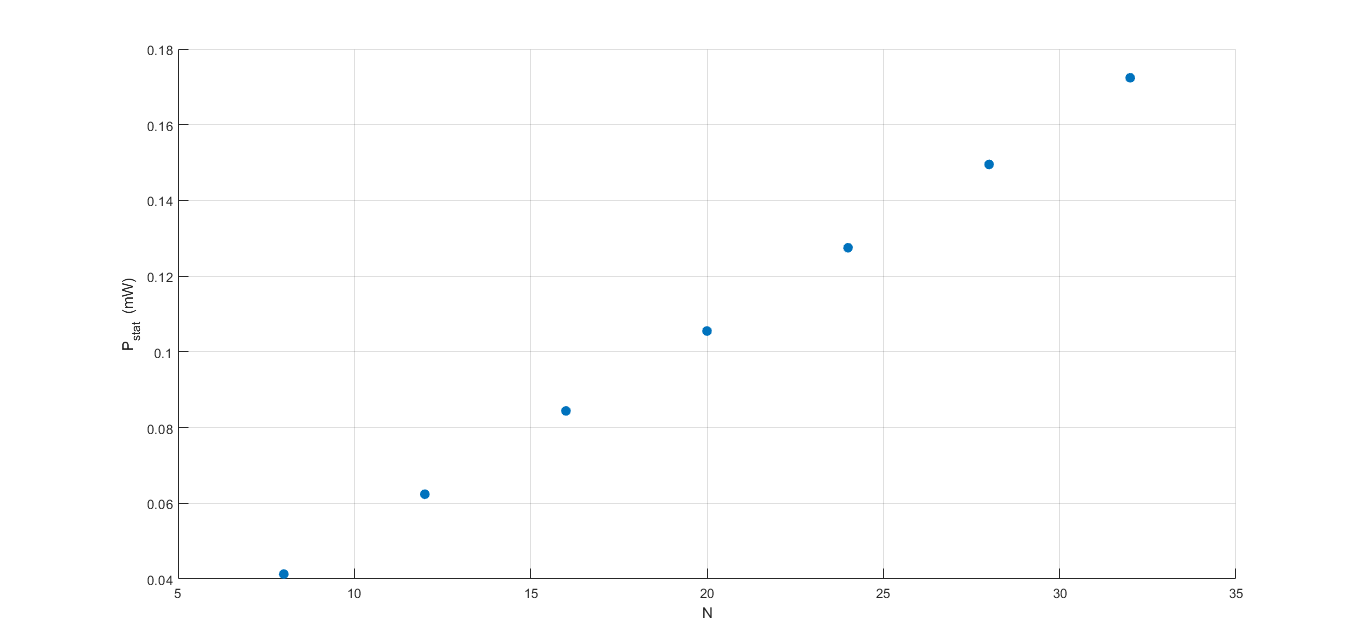
\includegraphics[width = 14 cm]{pentium/result_Pstat.png}
\caption{Static power Pentium IV as a function of $N$}
\label{result_Pstat}
\end{figure}

\begin{figure}[H]
\centering
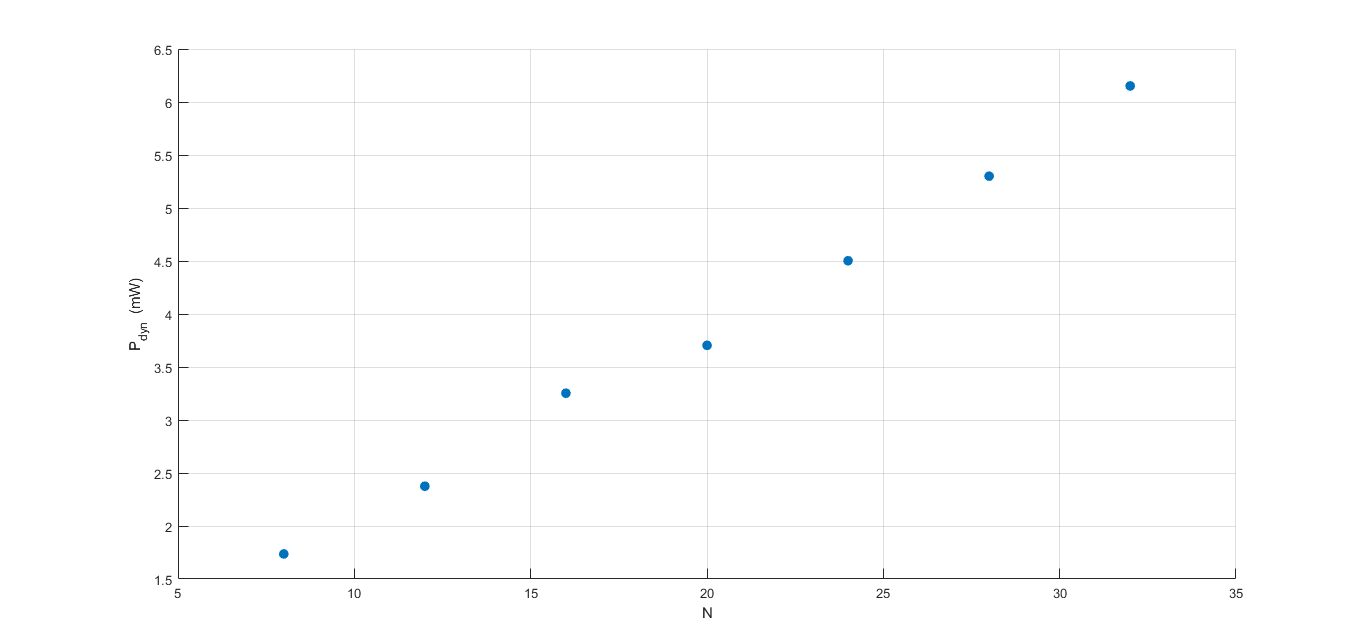
\includegraphics[width = 14 cm]{pentium/result_Pdyn.png}
\caption{Dynamic power Pentium IV as a function of $N$}
\label{result_Pdyn}
\end{figure}

\begin{figure}[H]
\centering
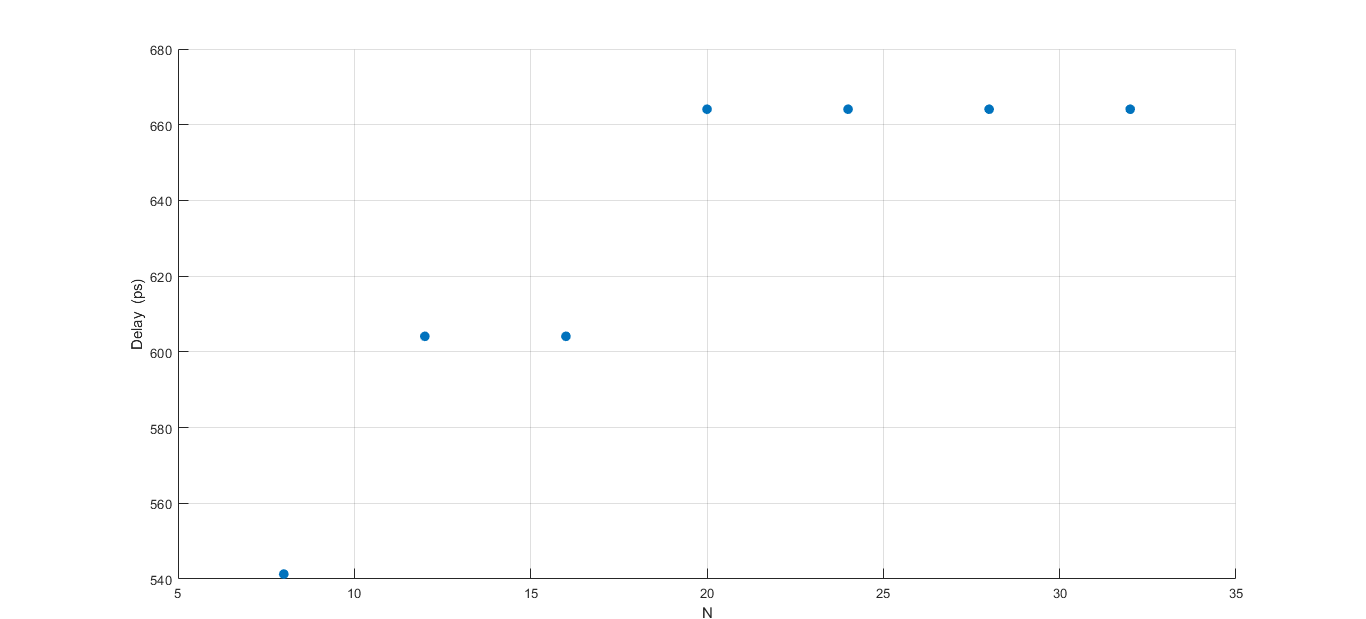
\includegraphics[width = 14 cm]{pentium/result_delay.png}
\caption{Delay without load Pentium IV as a function of $N$}
\label{result_delay}
\end{figure}


